\hypertarget{contas-puxfablicas-estadual}{%
\chapter{Contas Públicas Estadual}\label{contas-puxfablicas-estadual}}

O resultado primário do estado até o quarto bimestre de 2020 foi de
cerca de R\$ 1,08 bilhões, valor 73\% maior que o resultado primário no
mesmo período de 2019, quando foi pouco mais de R\$ 622 milhões. Veja o
Quadro \ref{resultado_primario} para mais detalhes sobre o resultado
primário.

As receitas primárias cresceu 10\% no quarto bimestre de 2020, como
mostra a Figura \ref{fig:var_receita_despesa_primaria}. As despesas
primárias cresceu 2,03\%. No quarto bimestre de 2019 as receitas tinham
crescido 9,55\% e as despesas 6,48\%. Comparando o crescimento das
despesas primárias no quarto bimestre de 2020 a taxa de crescimento foi
menor que em 2019. O baixo crescimento da despesas contribuiu para um
superávit primário de pouco mais de R\$ 1,08 bilhões até o quarto
bimestre de 2020.

A Figura \ref{fig:var_despesa_categoria} exibe as despesas por
categorias. Destaque para as despesas com assistência social, que
cresceu cerca de 133\% no quarto bimestre de 2020. Previdência social,
saúde e judiciário cresceu 16,2\%, 12,9\% e 18,8\% respectivamente. Por
outro lado, administração, segurança pública e educação recuaram.

\begin{smbox}[label={resultado_primario}, nameref={O que é o resultado primário}]{O que é o resultado primário}
O resultado primário é um dos principais indicadores das contas públicas, representa o esforço fiscal para diminuir o estoque da dívida. Ele é resultado da diferença entre as receitas e despesas (excluindo as receitas e despesas com juros). O superávit primário ou resultado primário positivo ocorre quandos as receitas primárias é maior que as despesas primárias. Indica a economia do governo para pagamento da dívida. O inverso, quando despesas primárias excedem as receitas primárias há déficit primário ou resultado primário negativo, incorrendo em aumento da dívida.
\end{smbox}

\begin{figure}[!h]
	\begin{subfigure}{\linewidth}
		\caption{\label{fig:var_receita_despesa_primaria}Variação da receita e despesa primária}
		\subcap{Variação acumulada (base: igual período do ano anterior)}
		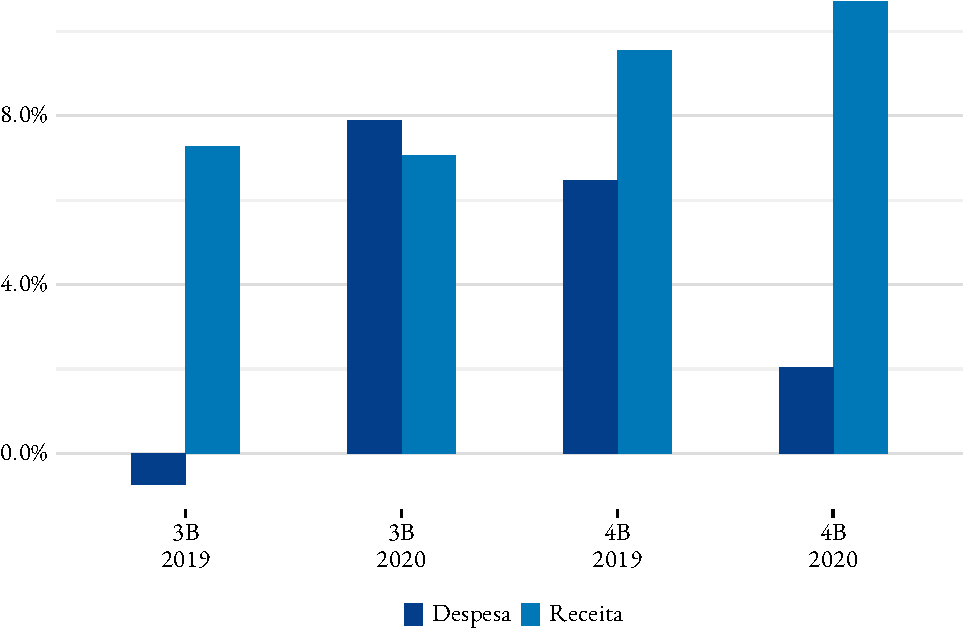
\includegraphics{fig/var_receita_despesa_primaria-1.pdf}
		\source{\abbr{siconfi}/Tesouro Nacional}
		\notes{\bimestres[3-4]}
	\end{subfigure}
	\begin{subfigure}{\linewidth}
		\caption{\label{fig:var_despesa_categoria}Variação da despesa por categoria}
		\subcap{Variação acumulada (base: igual período do ano anterior)}
		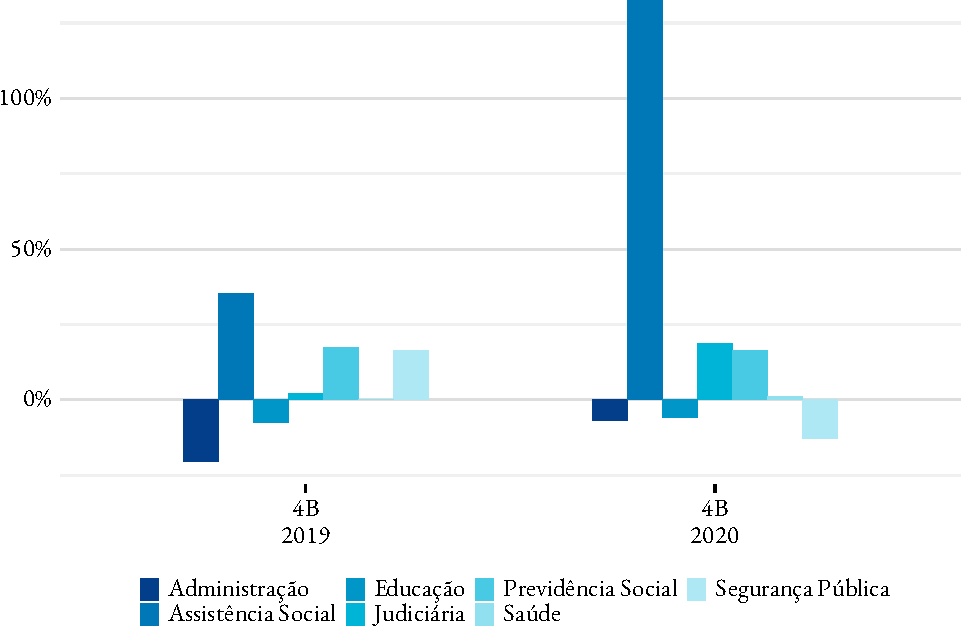
\includegraphics{fig/var_despesa_categoria-1.pdf}
		\source{\abbr{siconfi}/Tesouro Nacional}
		\notes{\bimestres[4]}
	\end{subfigure}
	\begin{subfigure}{\linewidth}
		\caption{\label{fig:desp_pessoal_rcl}Despesa total com pessoal em relação à RCL}
		\subcap{RCL e despesa acumulada até agosto}
		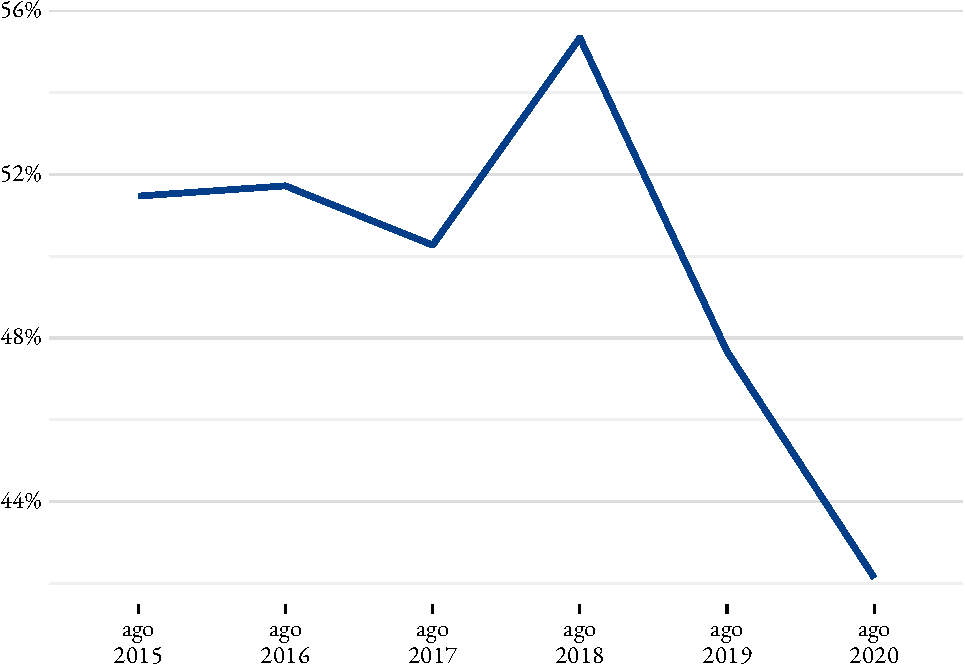
\includegraphics{fig/desp_pessoal_rcl-1.pdf}
		\source{\abbr{siconfi}/Tesouro Nacional}
	\end{subfigure}
\end{figure}

Despesas com pessoal em relação a receita corrente líquida (\abbr{rcl}),
conforme Figura \ref{fig:desp_pessoal_rcl}, encontra-se em 42,1\% em agosto
de 2020, valor abaixo do limite máximo de 49\% estabelecido na Lei de
Responsabilidade Fiscal (\abbr{lrf}) para o poder Executivo
\footnote{A \abbr{rcl}, de acordo com a \abbr{lrf}, deve ser apurada somando-se as receitas arrecadadas no mês em referência e nos onze anteriores. No entanto, pelo fato  dessa publicação cobrir dados até cerca do primero semestre optou-se pela utilização da \abbr{rcl} acumulada até o respectivo bimestre}.
Em agosto de 2015 a \abbr{rcl} destinada ao pagamento de pessoal
correspondia a 51,5\%, valor acima do limite máximo. O comprometimento
da \abbr{rcl} ao pagamento de pessoal extrapolou o limite em 2015, 2016,
2017 e 2018.

A dívida consolidada líquida (\abbr{dcl}) do estado em proporção a
\abbr{rcl} até agosto apresentou queda. Em agosto de 2020 essa indicador
ficou em 44,1\%, valor abaixo do limite definido pelo Senado Federal
para os estados, de duas vezes a \abbr{rcl}. Entre 2017 e 2018 a
\abbr{dcl} em proporção à \abbr{rcl} aumentou, saindo de 30\% para
52,3\% em 2019, conforme Figura \ref{fig:divida_rcl}.

\begin{figure}[!h]
	\begin{subfigure}{\linewidth}
		\caption{\label{fig:divida_rcl}Dívida Consolidada Líquida em relação à RCL}
		\subcap{RCL e DCL acumulada até agosto}
		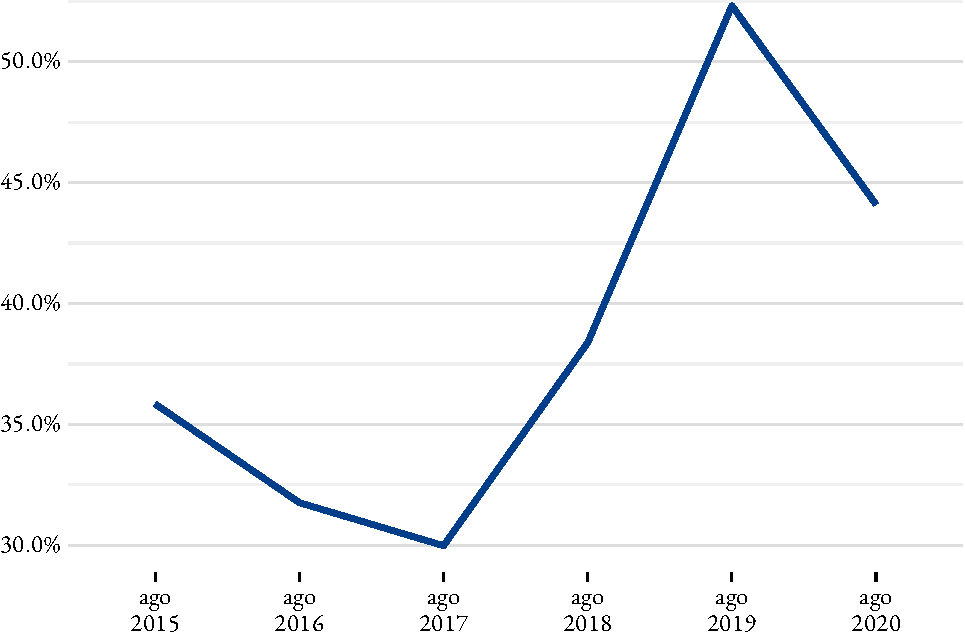
\includegraphics{fig/divida_rcl-1.pdf}
		\source{\abbr{siconfi}/Tesouro Nacional}
	\end{subfigure}
\end{figure}

O indicador da capacidade de pagamento (\abbr{capag}) do estado traz
informações a cerca da situação fiscal dos estados e municípios. O
índice é composto por três componentes: endividamento, poupança corrente
e liquidez. Estados e municípios recebem uma nota final, A, B, C ou D.

O Tocantins ficou com nota C em 2019 e 2020. Mesmo mantendo a mesma nota
entre 2019--2020, apresentou pioras em todos os indicadores. O
envididamento do estado que representa a \abbr{dcl} em proporção à
\abbr{rcl} saltou de 46,35\% para 67,6\%. A poupança corrente que
corresponde despesas corrente e receitas correntes ajustadas
(\abbr{rca}) também mostrou uma leve piora, saindo de 94,56\% para
95,9\%. A liquidez do estado cresceu de 539,4\% para 577,5\% em 2020.

Endividamento e poupança corrente estão em melhor condição, pois estão
mais próximo do limite para receber uma melhor nota. Para obter uma nota
A no índice de endividamento o estado deve conservá-lo abaixo de 60\%,
atualmente está em 67,6\%. A poupança corrente recebeu nota C em 2020
conforme Tabela \ref{tab:capag_uf}. Uma elevação na nota da poupança
corrente para B requer uma relação despesas correntes e \abbr{rca} menor
que 95\%, em 2020 ficou em 95,85\%. A liquidez do estado encontra-se em
situação mais delicada, em 2020 fechou em 577,5\%, valor quase cinco
vezes acima do limite para tirar nota A.

Dentre os estados da região norte, Tocantins e Roraima foram os que
apresentaram pior desempenho, conforme disposto na Tabela
\ref{tab:capag_uf}. Rondônia aparece com a melhor perfomance, saiu da
nota B para A entre 2019--2020. A redução no endividamento e na liquidez
garantiu nota A em todos os indicadores.

\begin{table}

\caption{\label{tab:capag_uf}Nota dos indicadores da CAPAG}
\subcap{Indicadores da CAPAG}
\begin{tabu} to \linewidth {>{\raggedright}X>{\centering}X>{\centering}X>{\centering}X>{\centering}X>{\centering}X>{\centering}X}
\toprule
\multicolumn{1}{c}{ } & \multicolumn{2}{c}{Endividamento} & \multicolumn{2}{c}{\makecell[c]{Poupança\\Corrente}} & \multicolumn{2}{c}{Liquidez} \\
\cmidrule(l{3pt}r{3pt}){2-3} \cmidrule(l{3pt}r{3pt}){4-5} \cmidrule(l{3pt}r{3pt}){6-7}
UF & 2019 & 2020 & 2019 & 2020 & 2019 & 2020\\
\midrule
AC & B & B & B & B & A & A\\
AM & A & A & B & B & A & A\\
AP & B & B & A & A & A & -\\
PA & A & A & B & B & A & A\\
RO & B & A & A & A & C & A\\
RR & A & A & A & A & C & C\\
TO & A & B & B & C & C & C\\
\bottomrule
\end{tabu}
\source{Boletim de Finanças dos Entes Subnacionais, 2019–-2020/Tesouro Nacional}
\notes{Amapá teve nota suspensa}
\end{table}
